\pdfoutput=1
\documentclass[11pt,a4paper]{article}
\usepackage{abhijit-research}
\renewcommand{\PaperCode}{P06}
\renewcommand{\PaperKind}{RESEARCH PAPER}
\renewcommand{\PaperVersion}{VERSION 1.1}
\renewcommand{\PaperDate}{AUGUST 2026}
\renewcommand{\PaperTitle}{Arity-Indexed Refinement Posets}
\renewcommand{\PaperSubtitle}{Forced Inverses and Rotational Root Geometry}
\renewcommand{\PaperFullTitle}{Arity-Indexed Refinement Posets, Forced Inverses, and Rotational Root Geometry}
\renewcommand{\PaperShortTitle}{Arity-Indexed Refinement}
\renewcommand{\PaperKeywords}{refinement poset; Stirling numbers; Mobius inversion; Fuss-Catalan numbers; real-rootedness; interlacing}
\renewcommand{\PaperClassification}{Counting, reachability, recursion, factorization, and conservation statements are exact. General root and sign laws beyond proved cases are identified as finite evidence and conjecture, not universal theorem.}
\renewcommand{\PaperCitation}{Singh, Abhijit. 2026. \textit{Arity-Indexed Refinement Posets, Forced Inverses, and Rotational Root Geometry}. Research manuscript, version 1.0.}
\begin{document}
\MakeResearchTitle
\MakeResearchContents
\MakeResearchAbstract{%
Exhaustive replacement of one terminal by $n$ unordered resultants generates arity-specific occurrence counts, multifactorial history counts, Fuss-Catalan forms, exact Kraft equality, and an orbit-stabilizer conservation law. Partial distinguishability states form the subposet of set partitions whose block count is congruent to one modulo $n-1$. Incidence inversion on this subposet produces an arity-indexed family of forced inverse sequences; the familiar binary factorial values are one member. The associated characteristic polynomial factors through $t^{n-1}$, spreading each positive reduced root over $n-1$ rotational rays. Parallel residue families, interlacing, sign alternation, and the root-at-one congruence are recorded with exact finite scope. An executable package passes 85 tests. The four prime-transparent arities within the terminal carrier are related to the four return-sector labels, while the stronger prime-closure ladder remains conjectural.
}
\section{One exhaustive replacement rule}
Begin with one terminal occurrence. At each application choose one current terminal and replace it by $n$ unordered resultants. Histories are retained separately; they are not aggregated by final form.

After $j$ applications the number of current occurrences is
\begin{equation}
L_j=1+j(n-1).
\end{equation}
The labelled history count obeys
\begin{equation}
H_{j+1}=L_jH_j,\qquad H_0=1,
\end{equation}
so
\begin{equation}
\boxed{H_j=\prod_{i=0}^{j-1}\bigl(1+i(n-1)\bigr).}
\end{equation}
For $n=2$ this is $j!$; for $n=3$ it is $(2j-1)!!$.

The number of unlabelled full $n$-ary forms after $j$ applications is the Fuss-Catalan number
\begin{equation}
F_{n,j}=\frac{1}{(n-1)j+1}\binom{nj}{j}.
\end{equation}
Forms reached by exactly one history number $n^j$.

\section{Kraft and orbit conservation}
Every completed form satisfies the exact base-$n$ Kraft equality
\begin{equation}
\sum_{\ell\in\operatorname{leaves}}n^{-\operatorname{depth}(\ell)}=1.
\end{equation}
For every symmetry class at depth $j$,
\begin{equation}
\boxed{|\Aut(T)|\,|\operatorname{Orb}(T)|=(n!)^j.}
\end{equation}
The executable audit verifies this to the declared finite boundaries for arities two through five.

\section{Growth regimes}
Occurrence count is linear in $j$, form count is exponential with asymptotic base $n^n/(n-1)^{n-1}$, the symmetry budget $(n!)^j$ is exponential, and history count is superexponential. At low arity forms eventually outgrow the symmetry budget; at higher arity the relation reverses. This crossover is a property of the exhaustive replacement system, not a new arithmetic operation.

\section{Reachable partition subposets}
A partial report is a partition of the presented resultants. One $n$-ary refinement splits one block into $n$, raising block count by $n-1$. Therefore the reachable ranks are exactly
\begin{equation}
\boxed{k\equiv1\pmod{n-1}.}
\end{equation}
At an admissible rank $k$, the number of partitions of a $q$-element carrier is still the Stirling number $\left\{\begin{smallmatrix}q\\k\end{smallmatrix}\right\}$. Arity changes reachability, not the census at a reachable rank.

\section{Forced incidence inverse}
Define $\mu_k^{(n)}$ on admissible ranks by
\begin{equation}
\mu_1^{(n)}=1,
\end{equation}
\begin{equation}
\sum_{\substack{j\le k\\j\equiv1\,(n-1)}}
\left\{\begin{matrix}k\\j\end{matrix}\right\}\mu_j^{(n)}=0
\qquad(k>1\text{ admissible}).
\end{equation}
This is the incidence inverse of the arity-restricted refinement poset.

\begin{table}[H]\centering
\caption{First forced inverse values on admissible ranks.}
\begin{tabular}{cl}
\toprule
arity $n$ & $\mu_k^{(n)}$\\\midrule
2 & $1,-1,2,-6,24,-120,720,\ldots$\\
3 & $1,-1,24,-3060,1249920,-1253750400,\ldots$\\
4 & $1,-1,349,-2018016,77366328753,\ldots$\\
5 & $1,-1,6950,-2491030400,\ldots$\\
6 & $1,-1,179486,-5191034942731,\ldots$\\
\bottomrule
\end{tabular}
\end{table}
The binary factorial sequence is one member of a larger arity-indexed family. Strict sign alternation was computationally verified through the declared finite range; a universal proof is a separate obligation.

\section{Characteristic polynomial}
For a carrier with $q$ presented resultants define
\begin{equation}
C_q^{(n)}(t)=
\sum_{\substack{k\le q\\k\equiv1\,(n-1)}}
\left\{\begin{matrix}q\\k\end{matrix}\right\}\mu_k^{(n)}t^{q-k}.
\end{equation}
All exponents lie in one residue class modulo $n-1$, hence
\begin{equation}
\boxed{C_q^{(n)}(t)=t^aD_q^{(n)}(t^{n-1}),\qquad a\equiv q-1\pmod{n-1}.}
\end{equation}
A positive root $u$ of $D_q^{(n)}$ generates roots of $C_q^{(n)}$ on the $n-1$ rays
\begin{equation}
\arg t=\frac{2\pi r}{n-1},\qquad r=0,\ldots,n-2.
\end{equation}
The binary positive-real geometry is the one-ray degeneration.

\begin{table}[H]\centering
\caption{Audited reduced polynomials at $q=7$.}
\begin{tabular}{cll}
\toprule
$n$ & $D_7^{(n)}(u)$ & positive roots\\\midrule
3 & $u^3-301u^2+3360u-3060$ & $1,10.573,289.427$\\
4 & $u^2-350u+349$ & $1,349$\\
5 & $u-140$ & $140$\\
\bottomrule
\end{tabular}
\end{table}

\begin{figure}[H]\centering
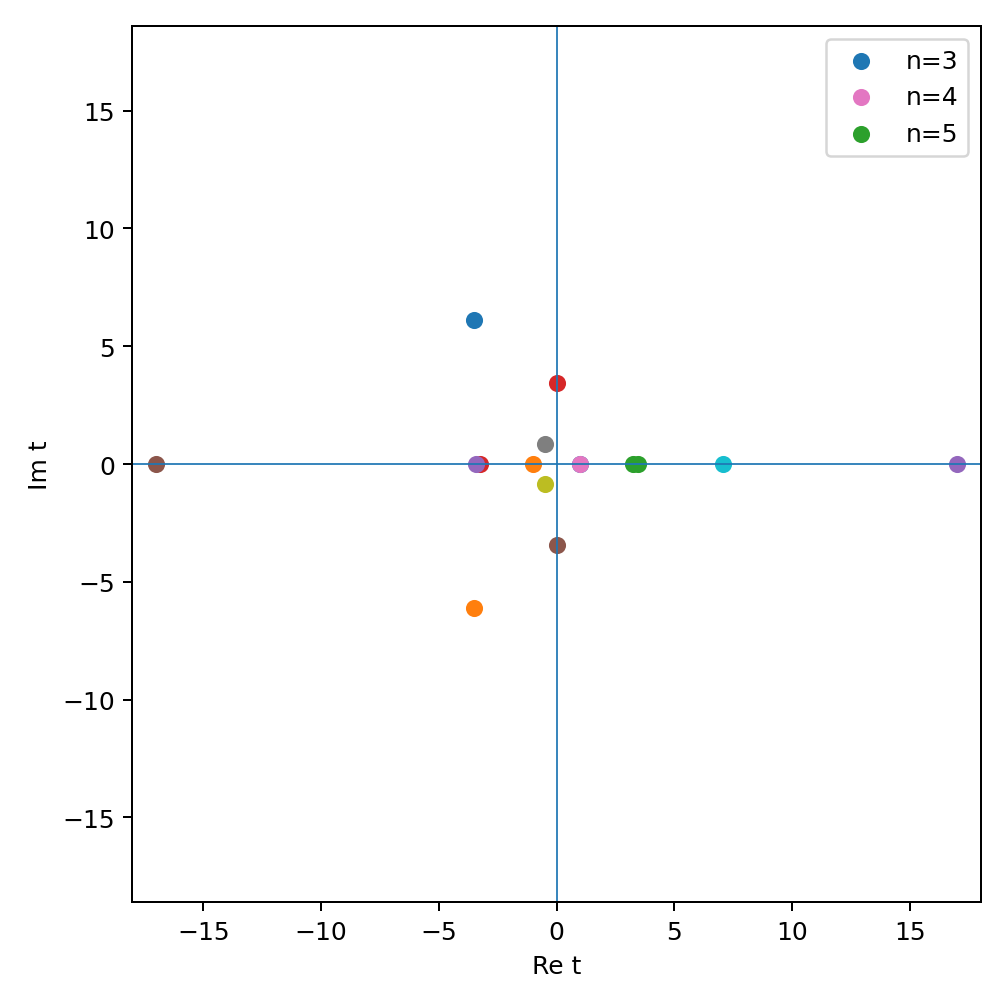
\includegraphics[width=.64\linewidth]{figures/p6_rotational_roots.png}
\caption{Rotational root rays generated from audited positive reduced roots.}
\end{figure}

\section{Parallel families and root at one}
At each arity there are $n-1$ residue families indexed by $q\bmod(n-1)$. The finite audit displays interlacing within each family. The audited rule
\begin{equation}
D_q^{(n)}(1)=0\quad\Longleftrightarrow\quad q\equiv1\pmod{n-1}
\end{equation}
holds throughout the computed domain. A general theorem requires a recurrence preserving real stability or a total-positivity argument for the restricted Stirling transform.

\section{Transparent prime sectors in the observer carrier}
On the finite nonterminal index set $\{2,\ldots,9\}$, the transparent arities are exactly
\begin{equation}
\{2,3,5,7\}.
\end{equation}
They label four prime/composite return sectors under $d\mapsto1-d\pmod {10}$. This gives a generated role for the prime indices: they are the irreducible arities whose intermediate binomial capacities vanish in their own modulus. The composite partners record either squarefree coupling ($6=2\cdot3$) or repeated occupation ($4,8,9$).

The stronger notebook conjecture that every genuinely new observer-closure rank must be prime is not proved by this finite pattern. A valid theorem would require a fixed role-generation rule that predicts the next closure rank before testing primality. The present exact result is narrower: prime transparency selects the four sector labels, and the nine-state carrier organizes their pair relations into a 36-cell frontier.

\section{What is proved and what is finite evidence}
The occurrence, history, Fuss-Catalan, Kraft, orbit-stabilizer, reachability, Stirling-census, inverse-recursion, and residue-factorization statements are exact. General real-rootedness, sign alternation, interlacing, and the root-at-one rule outside the proved binary case are retained as computationally supported conjectures unless and until universal proofs are supplied.

\section{Executable audit}
The supplied perspective-arity package passes 85 tests. It checks exhaustive constructors, independent closed forms, refinement inverses, symmetry conservation, capacity identities, prime transparency, groupoid lifts, and negative controls. Numerical roots are computed only after exact integer coefficients are established.


\section{Complete counting derivations}
After $j$ applications of an $n$-resultant replacement, the number of current occurrences is
\begin{equation}
L_j=1+j(n-1).
\end{equation}
At the next step any current occurrence may be selected, so the number of labelled histories obeys
\begin{equation}
H_{j+1}=L_jH_j,\qquad H_0=1,
\end{equation}
and therefore
\begin{equation}
H_j=\prod_{i=0}^{j-1}[1+i(n-1)].
\end{equation}
For $n=2$ this is $j!$; for $n=3$ it is $(2j-1)!!$. The number of unlabelled full $n$-ary forms with $j$ internal occurrences is the Fuss--Catalan number
\begin{equation}
F_{n,j}=\frac{1}{(n-1)j+1}\binom{nj}{j}.
\end{equation}
The finite constructor exhaustively reproduced, among other values, $285$, $2530$, and $23751$ for $n=5$.

For every completed form,
\begin{equation}
\sum_{\ell\in\mathrm{leaves}}n^{-\operatorname{depth}(\ell)}=1.
\end{equation}
This follows by induction because replacing one leaf of weight $n^{-d}$ by $n$ children of weight $n^{-(d+1)}$ preserves the sum. Every internal occurrence also contributes one independent permutation of its resultants, so orbit--stabilizer gives
\begin{equation}
|\Aut(T)|\,|\operatorname{Orb}(T)|=(n!)^j.
\end{equation}

\section{Reachable ranks and forced inverse}
One replacement increases block count by $n-1$. Hence reachable partition ranks satisfy
\begin{equation}
k\equiv1\pmod{n-1}.
\end{equation}
At an admitted rank the number of partitions remains the ordinary Stirling number. The incidence inverse is forced by
\begin{equation}
\mu_1^{(n)}=1,\qquad
\sum_{\substack{j\le k\\j\equiv1\ (n-1)}}
\left\{\begin{matrix}k\\j\end{matrix}\right\}\mu_j^{(n)}=0.
\end{equation}
The first values are
\begin{center}
\begin{tabular}{cl}
\toprule
$n$&inverse on admitted ranks\\\midrule
2&$1,-1,2,-6,24,-120,\ldots$\\
3&$1,-1,24,-3060,1249920,\ldots$\\
4&$1,-1,349,-2018016,\ldots$\\
5&$1,-1,6950,-2491030400,\ldots$\\
6&$1,-1,179486,-5191034942731,\ldots$\\
\bottomrule
\end{tabular}
\end{center}
The alternating signs were checked through admitted rank 31 in the supplied finite audit. Only the binary member reduces to factorials.

\section{Rotational characteristic geometry}
Define
\begin{equation}
C_q^{(n)}(t)=
\sum_{\substack{k\le q\\k\equiv1\ (n-1)}}
\left\{\begin{matrix}q\\k\end{matrix}\right\}\mu_k^{(n)}t^{q-k}.
\end{equation}
All exponents occupy one residue class, so
\begin{equation}
C_q^{(n)}(t)=t^aD_q^{(n)}(t^{n-1}),
\qquad a\equiv q-1\pmod{n-1}.
\end{equation}
A positive root $u$ of $D$ produces $n-1$ roots on rays $\arg t=2\pi r/(n-1)$. At $q=7$ the audited reduced polynomials are
\begin{center}
\begin{tabular}{cll}
\toprule
$n$&$D_q^{(n)}(u)$&positive roots\\\midrule
3&$u^3-301u^2+3360u-3060$&$1,10.573,289.427$\\
4&$u^2-350u+349$&$1,349$\\
5&$u-140$&$140$\\
\bottomrule
\end{tabular}
\end{center}
Finite calculations show parallel residue families and a root at one when $q\equiv1\pmod{n-1}$. A universal proof of reduced real-rootedness and interlacing remains a stated theorem target; the manuscript does not replace that proof with plots.

\section{Reproducibility envelope}
The archive constructs histories and forms independently, checks the closed counts, verifies Kraft equality and orbit products, computes the forced inverses as exact integers, constructs characteristic polynomials, and extracts roots. Floating-point root plots are evidence only; a proof-quality computation should add exact Sturm isolation or certified interval arithmetic.

\begin{thebibliography}{99}
\bibitem{stanley} R. P. Stanley, Enumerative Combinatorics, Volumes 1 and 2, Cambridge University Press.
\bibitem{rota} G.-C. Rota, On the foundations of combinatorial theory I: theory of Mobius functions, Zeitschrift fuer Wahrscheinlichkeitstheorie 2 (1964), 340--368.
\bibitem{fuss} N. I. Fuss, Solutio quaestionis, quot modis polygonum, Nova Acta Academiae Scientiarum Imperialis Petropolitanae 9 (1791), 243--251.
\bibitem{brenti} F. Brenti, Unimodal, log-concave and Polya frequency sequences in combinatorics, Memoirs of the American Mathematical Society 81 (1989).
\end{thebibliography}
\end{document}
